\documentclass[a4paper, 12pt]{article}%тип документа

%отступы
\usepackage[left=2cm,right=2cm,top=2cm,bottom=3cm,bindingoffset=0cm]{geometry}

%Русский язык
\usepackage[T2A]{fontenc} %кодировка
\usepackage[utf8]{inputenc} %кодировка исходного кода
\usepackage[english,russian]{babel} %локализация и переносы

%Вставка картинок
\usepackage{wrapfig}
\usepackage{graphicx}
\graphicspath{{pictures/}}
\DeclareGraphicsExtensions{.pdf,.png,.jpg}

%оглавление
\usepackage{titlesec}
\titlespacing{\chapter}{0pt}{-30pt}{12pt}
\titlespacing{\section}{\parindent}{5mm}{5mm}
\titlespacing{\subsection}{\parindent}{5mm}{5mm}
\usepackage{setspace}

%Графики
\usepackage{multirow}
\usepackage{pgfplots}
\pgfplotsset{compat=1.9}

%Математика
\usepackage{amsmath, amsfonts, amssymb, amsthm, mathtools}

%Стиль страницы
\usepackage{fancyhdr}
\pagestyle{fancy}

\begin{document}

\begin{titlepage}

\begin{center}
%\vspace*{1cm}
\large\textbf{Московский Физико-Технический Институт}\\
\large\textbf{(национальный исследовательский университет)}
\vfill
\line(1,0){430}\\[3mm]
\huge\textbf{Лабораторная работа №77}\\
\line(1,0){430}\\[1mm]
\vfill
\large Баканова К.В., Б01-003\\
%\vspace*{1cm}
\large март 2022 г.\\
\end{center}

\end{titlepage}
\fancyhead[L] {Лабораторная работа №77}
\noindent \textbf{Цель работы:} \\
\indent Изучение операционных усилителей и схем на их основе.\\
\noindent \textbf{В работе используются:} \\
\indent Операционный усилитель, резисторы, генератор напряжения, осциллограф.

\section{Ход работы}

\subsection{Измерение коэффициента усиления ОУ}
\fancyhead[L] {Лабораторная работа №77}
\fancyhead[R] {Баканова К.В.}

\begin{enumerate}

\item Соберем схему изображенную на рис.1. Возьмем резисторы сопротивлением $R_1 = R_2 = R_3 = 100$ кОм и $R_4 = 1$ кОм.

\begin{figure}[h]
\begin{center}
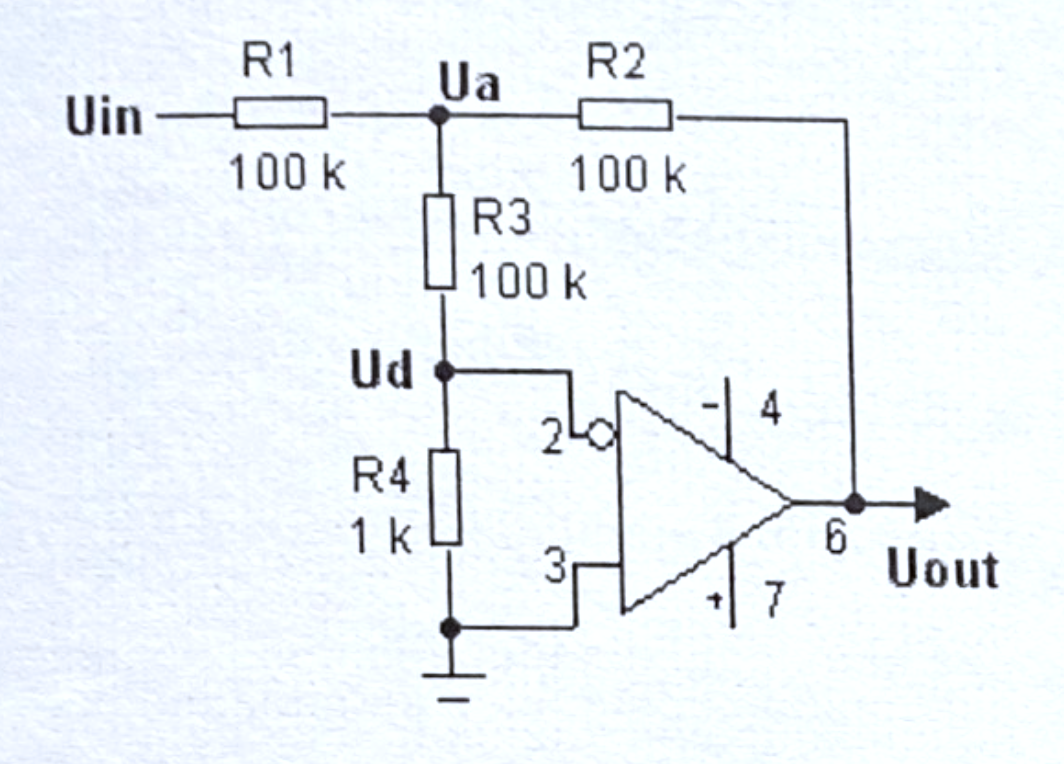
\includegraphics[width = 0.7\textwidth]{scheme1.png}
\caption{Схема измерения коэффициента усиления}
\end{center}
\end{figure}

\item Подадим на вход колебание с амплитудой $U = 2$ В и частотой $f = 10$ Гц. Измерим величину напряжений $U_a$ и $U_{out}$:

\[U_{out} = 1,4 \: \text{В}\]

\[U_a = 2 \: \text{мВ}\]

\item Рассчитаем коэффициент усиления операционного усилителя по формуле:

\[A_0 = (1 + \frac{R_3}{R_4}) \cdot \frac{U_{out}}{U_a} \simeq 7 \cdot 10^4\]

\end{enumerate}

\subsection{Амплитудно-частотная характеристика ОУ}
\fancyhead[L] {Лабораторная работа №77}

\begin{enumerate}

\item Для схемы на рис. 1 снимем зависимость коэффициента усиления от частоты:

\begin{center}
\begin{tabular}{|c|c|c|c|c|c|c|c|c|c|c|}
\hline 
A & 24000 & 12200 & 6300 & 2550 & 1265 & 636 & 257 & 129 & 65 & 27 \\ 
\hline 
f, кГц & 0,05 & 0,1 & 0,2 & 0,5 & 1 & 2 & 5 & 10 & 20 & 50 \\ 
\hline 
\end{tabular} 
\end{center}

\item Построим снятую зависимость в двойном логарифмическом масштабе, откладывая частоту в герцах а коэффициент усиления в децибелах ($A_{\text{дБ}} = 20lgA$).

\begin{figure}[h]
\begin{center}
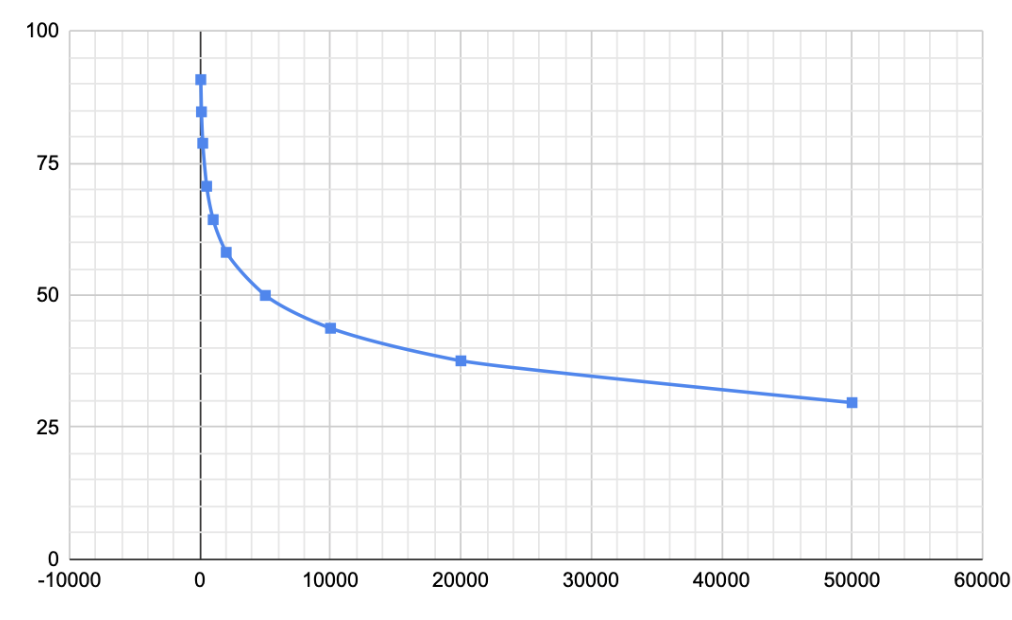
\includegraphics[width = 0.7\textwidth]{graph1.png}
\caption{АЧХ операционного усилителя}
\end{center}
\end{figure}

\item Экстраполировав график до пересечения с $A_0$ и 1 определим граничную частоту:

\[f = 0 \Rightarrow A_0 = 93,48\]

\[A = 1 \Rightarrow f_r = 162530 \: \text{Гц}\]

Из этого получаем, что $f_{p0} = 25,5 \: \text{Гц}$

\end{enumerate}

\newpage
\subsection{Неинвертирующий усилитель}
\fancyhead[L] {Лабораторная работа №77}

\begin{enumerate}

\item Соберем схему неинвертирущего усилителя (рис. 3). $R_1	= 1$ кОм, $R_2 = 100$ кОм.

\begin{figure}[h]
\begin{center}
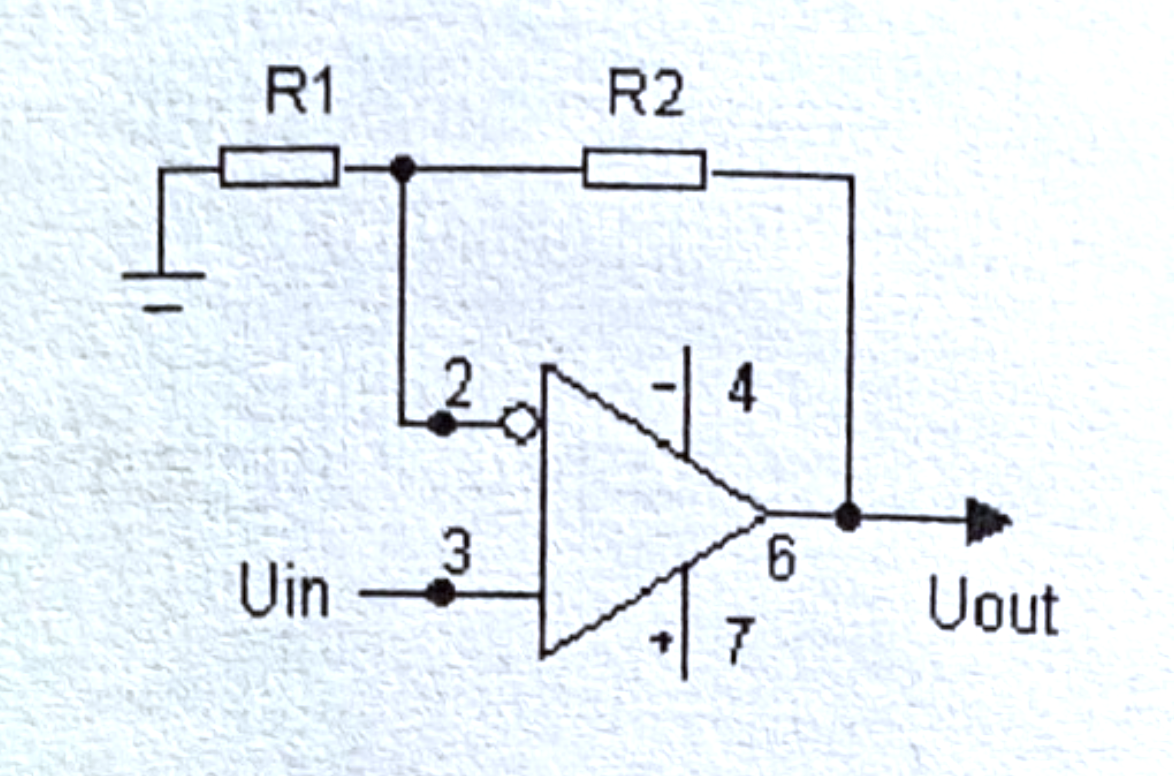
\includegraphics[width = 0.7\textwidth]{scheme2.png}
\caption{Схема неинвертирующего усилителя}
\end{center}
\end{figure}

\item Измерим постоянное напряжение на выходе $U_{out}$:

\[U_{out} = 1,26 \: \text{В}\]

\item Снимем зависимость коэффициента усиления от частоты K(f).

\begin{center}
\begin{tabular}{|c|c|c|c|c|c|c|c|c|c|c|c|}
\hline 
K(f) & 84 & 87 & 86 & 86 & 86 & 86 & 85 & 80 & 67 & 45 & 21 \\ 
\hline 
f, Гц & 10 & 50 & 100 & 200 & 500 & 1000 & 2000 & 5000 & 10000 & 20000 & 50000\\ 
\hline 
\end{tabular} 
\end{center}

По полученным данным построим график:

\begin{figure}[h]
\begin{center}
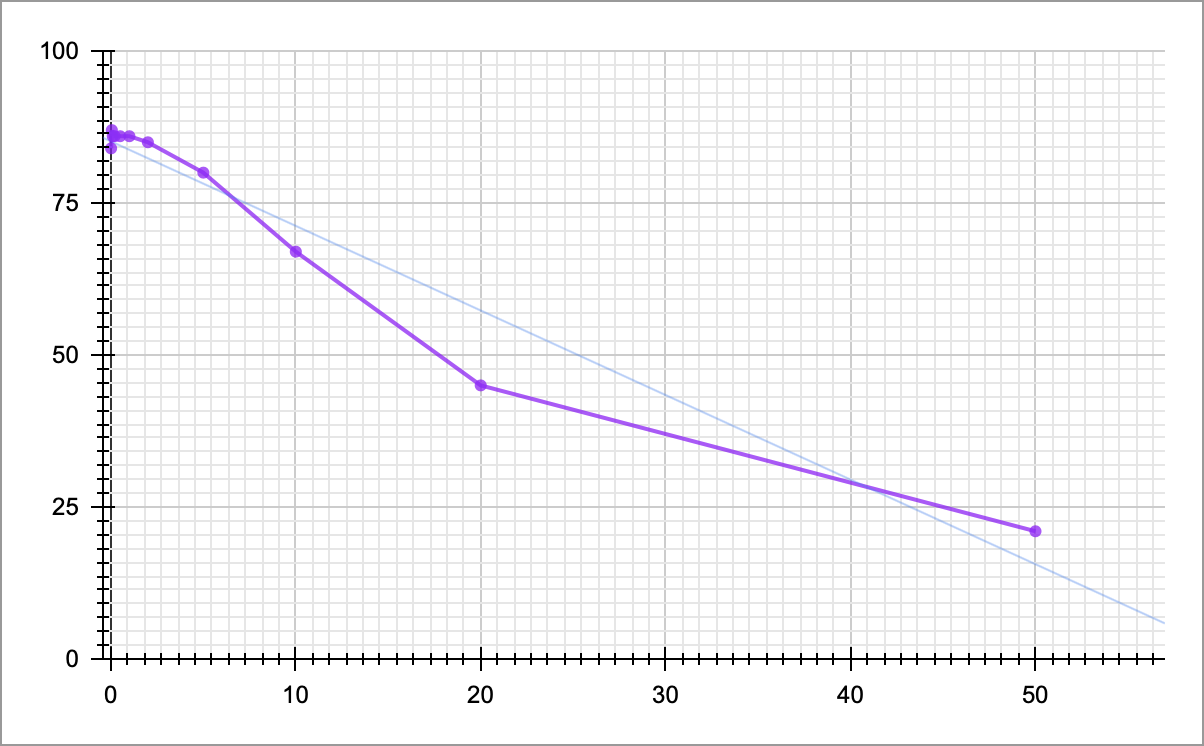
\includegraphics[width = 0.7\textwidth]{graph2.png}
\caption{Зависимость K(f) у неинвертирующего усилителя}
\end{center}
\end{figure}

Линейной приближения дало зависимость - $K = 90,16 - 0,0022f$.

\item Определим граничную частоту $F_p$ по уровню 0,7 - $K = 60,2$. Получается, что $F_p = 13,6$ кГц.

\item Определим максимальную амплитуду неискаженного выходного напряжения на низкой частоте $(f = 1$ кГц):

\[U_{max-l} = 6,4 \: \text{В}\]

\item Включим ОУ по схеме повторителя. Коэффициент передачи и усиления равен единице. Определим максимульную амплитуду неискаженного сигнала на частоте $f = 1$ МГц:

\[U_{max} = 0,6 \: \text{В}\]

\end{enumerate}

\newpage
\subsection{Инвертирующий усилитель}
\fancyhead[L] {Лабораторная работа №77}

\begin{enumerate}

\item Соберем схему инвертирующего усилителя используя те же резисторы, что в разделе 3, определим коэффициент усиления $K_0$ и граничную частоту $F_p$.

\begin{figure}[h]
\begin{center}
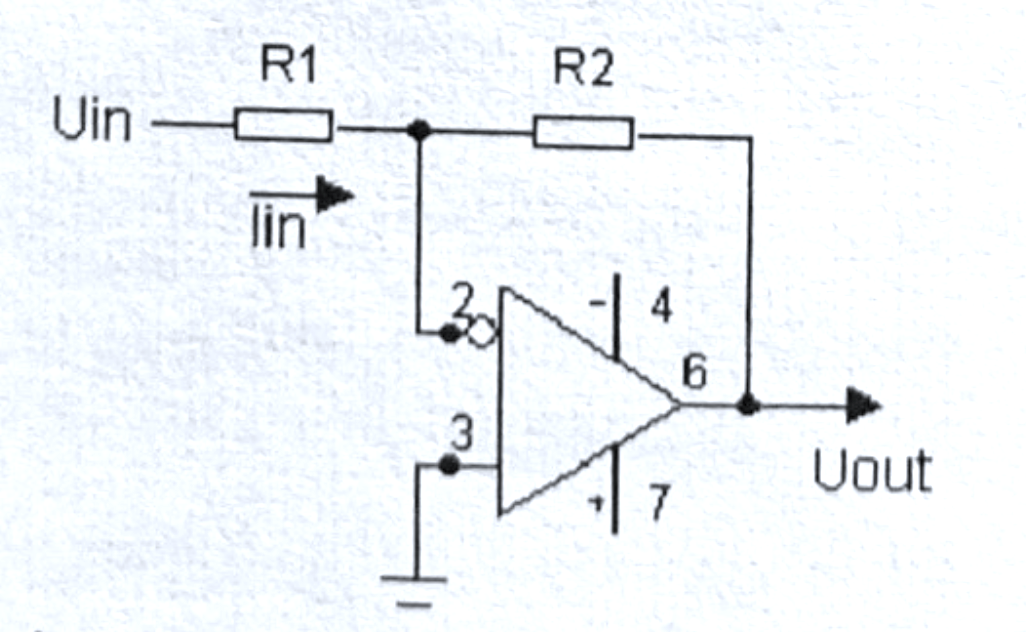
\includegraphics[width = 0.7\textwidth]{scheme3.png}
\caption{Схема инвертирующего усилителя}
\end{center}
\end{figure}

\item Убедимся, что коэффициент усиления $K_0 = -R_2 / R_1 \Rightarrow K_0$ = -90. Найдем частоту $F_p$ по уровню 0,7:

\[F_p = 13,6 \: \text{кГц},\]

она имеет то же значение, что и для неинвертирующего усилителя.

\end{enumerate}

\newpage
\subsection{Разностный усилитель}
\fancyhead[L] {Лабораторная работа №77}

\begin{enumerate}

\item Соберем схему, выбрав $R_3 = R_1 = 1$ кОм, $R_4 = R_2=10$ кОм.

\begin{figure}[h]
\begin{center}
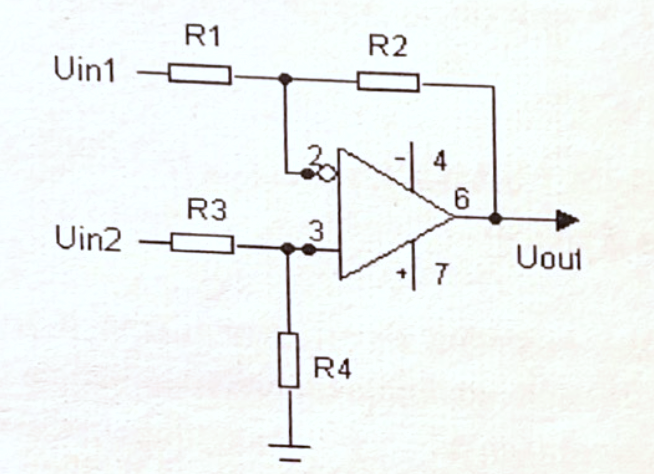
\includegraphics[width = 0.7\textwidth]{scheme4.png}
\caption{Схема разностного усилителя}
\end{center}
\end{figure}

\item Измерим коэффициент усиления сначала по входу 1, а затем по входу 2. При втором измерении вход $U_{in1}$ соединим с землей.
\[U_{in1} = 29,2 \: \text{мВ},\]
\[U_{in2} = 46,64 \: \text{мВ},\]
\item Объединим входы $U_{in1}$ и $U_{in2}$, убедимся, что коэффициент усиления синфазного сигнала близок к нулю.
\item Продемонстрируем, что для идеального ОУ выходное напряжение
\[U_{out} = (U_{in2}-U_{in1})*(R_2 / R_1)=174,4 \: \text{мВ.}\]
При этом экспериментальное значение 
\[U_{out exp} = 167,9 \: \text{мВ,}\]
что почти совпадает с вычисленным по формуле.

\end{enumerate}

\end{document}
